 \section{Dirichlet Variable Selection For Decision Trees: The DiVaS method}
\label{ch:var_select}

%subsection{Introduction}
Many data analysis procedures, originally designed for inference in low dimensional spaces, create difficulties when dealing with high dimensional data.  Often data analysts use low dimensional intuition and apply similar logic to high dimensional data, which can often lead to erroneous conclusions. The approach outlined in this thesis not only moves around the high dimensional space efficiently, but also indicates with a high degree of probability which covariates are useful in determining the response at the tree nodes. In addition, we retrieve summary data indicating which dimensions are useful assisting the data analyst in the interpretation of results. Our primary focus in this thesis is on inferring a structural relationship between dimensions and the response of interest, with a preference towards interpretability. 

There are perhaps two predominant approaches to dealing with high dimensional data. The first attempts to only include dimensions that are important based on some metric of choice, usually with a filter run over the data to screen out some dimensions. Examples of this are principal components analysis \cite{tipping1999probabilistic} and various other approaches surveyed by Dash and Liu \cite{dash1997feature}. The second approach attempts to fit a model to the best dimensions sequentially. Examples of this approach include forward, backward and stagewise searches for regression models \cite{miller1984selection} \cite{myers1990classical} \cite{berk1978comparing}. The lasso \cite{tibshirani1996regression} is a problem which can be considered in either category, depending upon the approach taken. If we use the LARS algorithm to fit the model for all values of $\lambda$ then the method can be considered iterative. If instead, we fit a model for the lasso objective function choosing a single value of $\lambda$, for example by cross validation, then the method can be thought of as a filtering approach. Our approach is similar to both approaches and operates by choosing a middle ground between these two extremes. As a byproduct of choosing this middle ground we are able to search the space of models more effectively and give intuitive summary results indicating which covariates are useful, while returning models to the analyst for use in prediction and inference. 

In this chapter we follow a \bayesorprob\ framework. We define a new prior measure over trees, which facilitates comparison across trees based on a global search of the tree space, and automatically induces coherent covariate selection. We assume a working familiarity with Markov chain Monte Carlo (MCMC) methods. For a good review of MCMC approaches to machine learning problems, we recommend the paper by Andrieu, De Freitas, Doucet and Jordan \cite{andrieu2003introduction}. We show through an example that greedily grown decision trees can fail to recover good trees in high dimensional data. Moreover, we find that previously implemented Bayesian approaches to decision tree learning have been applied only to low dimensional spaces \cite{chipman1998bayesian} \cite{gramacy2008bayesian} \cite{denison1998bayesian}. Applying the same approaches to high dimensional data is inappropriate and we demonstrate this through examples. These methods fail to move around the large dimensional space efficiently causing poor mixing and only finding local optima. 

Nearly all the previous approaches to decision tree induction have not explicitly incorporated model selection into the tree framework \cite{chipman1998bayesian} \cite{gramacy2008bayesian} \cite{denison1998bayesian} \cite{breiman1984classification} \cite{quinlan1993c4}. A notable exception is the recent paper by Gramacy and Taddy \cite{gramacy2012categorical} where binary indicators are used to perform model selection within a terminal node. Specifically, Gramacy and Taddy define a mixture of a Gaussian process (GP)\newabbrev{abbrev:GP} and the GP's limiting linear model, and use a point mass mixture to choose between the GP and the limiting linear model within each terminal node. This is in contrast with our approach, which aims to perform variable selection at the level of the decision tree itself and not for each model in each terminal node. Another notable exception is the work of Ishwaran, Kogalur, Gorodeski, Minn, and Lauer, who define a new quantity called a maximal subtree, and use the inherent topology of the tree and the maximal subtree to measure variable importance  \cite{ishwaran2010high}. Ishwaran et al. work in the context of random survival forests, built using bootstrapped data.  Most researchers have used implicit selection, for which predictors are chosen at the end of the greedy induction strategy as the predictors which are useful. Those not selected are considered not useful. Currently, most tree algorithms rely on a pruning rule for determining which covariates are useful. This implicit approach has the drawback of only providing ``yes/no'' answers to inclusion, and does not allow one to order the dimensions in some meaningful fashion. In our work we explicitly model these probabilities of inclusion and exclusion in the decision tree. This not only allows for useful predictor selection when choosing models, but also improves the efficiency of searching in large dimensions.  We note that we include a prune function in our proposal which affects the selection of useful covariates. However, in large dimensions, a better way to improve the efficiency of the searching algorithm is to treat covariates differently based on their utility in the model. 

This chapter follows from the original Bayesian decision tree model of Chipman, George and Mcculloch \cite{chipman1998bayesian} (referred to hereafter as CGM), and Gramacy and Lee \cite{gramacy2008bayesian}(hereafter referred to as GL)\newabbrev{abbrev:GL}. Specifically, we propose a generalization of the models used by CGM and of GL. We allow rotate moves at all permissible nodes of the tree and varying selection probabilities on each covariate. In this manuscript we confine ourselves to categorical response data. All results can easily be extended and applied similarly to continuous data. In addition, we study the approach of CGM to large dimensional datasets. To our knowledge, the largest dimensions of data that the aforementioned approaches have been studied on are at most 15 dimensions. We find our method to be more effective than the CGM approach for large dimensional data. We also study the efficacy of a general rotate move in the transition kernel of the Markov chain.

The remainder of this paper unfolds as follows. Section \ref{sec:related_work} reviews previous greedy and Bayesian approaches to decision tree learning. Section \ref{sec:model_details} shows our model and describes how this is a modification of the algorithm proposed by CGM \cite{chipman1998bayesian}. In this and the next chapter we place emphasis on the algorithmic details of our procedure and only briefly describe some of the mathematical properties. Section \ref{sec:ecc} states necessary conditions for consistency of the decision trees we propose. Section \ref{sec:ase} shows how high dimensional data can create problems for both greedy and Bayesian approaches that have been previously proposed, and gives an example. Section \ref{sec:real_data} applies our approach to a dataset taken from the UCI machine learning repository. In Section \ref{sec:conc} we state conclusions and point towards future work.

\subsection{Related Work}\label{sec:related_work}
Some of the most well known approaches to decision tree learning are two approaches invented in the 1980's; these are Breiman, Friedman, Olshen, and Stone's cart method \cite{breiman1984classification} and Quinlan's C4.5 algorithms and variants \cite{quinlan1993c4}.  
The work of Breiman et al. \cite{breiman1984classification} showed the practical and theoretical approaches to decision tree induction. In Breiman et al. \cite{breiman1984classification}, the theoretical framework for discussing decision trees is given in terms of general impurity functions, allowing results to apply to specific impurities suggested by Quinlan \cite{quinlan1993c4}. For a theoretical treatment of consistency, the work of Devroye, Lugosi, and Gy\"{o}rfi \cite{devroye1996probabilistic} provided the foundation and application of the theory to certain tree methods.

The consistency of tree classifiers was also discussed by Breiman et al. \cite{breiman1984classification}. They showed that, under fairly general conditions, tree classifiers are asymptotically consistent, meaning trees can recapture the correct classifier if they are given enough data. The practical problem with this is that we usually only have a finite amount of data. Although we do not overcome this practical limitation, the results in Section \ref{sec:ecc} improve the rate of convergence by exploiting sparsity. Quinlan's approach modified the impurity functions proposed by Breiman \cite{breiman1984classification}, and also allowed for multiway splits at nodes in the tree \cite{quinlan1993c4}. Empirically, we have found that the entropy impurity function approach of Quinlan \cite{quinlan1993c4} performs better if there is a difference, although there is usually little or no difference in terms of the final tree. 

In our probabilistic approach, we quantify \emph{a priori} uncertainty in the classifier with a prior probability measure over trees. By defining a prior over trees, we induce a posterior distribution over trees via Bayes' rule shown in Equation \ref{bayesrule}, where $\theta$ denotes parameters in the model and $D$ denotes observed data.

\begin{equation}\label{bayesrule}
\Pr(\theta \vert D ) = \frac{\Pr(D\vert \theta )\Pr(\theta)}{\Pr(D)}
\end{equation}

 The posterior allows us to \emph{search} the space of trees, which is distinctly different from the greedy induction approach. In the Bayesian approach to decision tree induction several researchers have proposed various methods for searching over the tree space. The space of trees is a large discrete space, so MCMC algorithms are usually applied to search this space. CGM  \cite{chipman1998bayesian} proposed a clever process prior on the tree space, denoted $\Pr(\mathcal{T})$, to induce a posterior which moves between a varying number of dimensions. 
 %avoiding Reversible Jump moves
  Let $\mathcal{T}$ denote the tree and $\theta$ the collection of parameters in each terminal node (mean or class probabilities) and $D$ denotes data. Applying Bayes' rule, we have the result 
 \begin{equation}
 \label{eqn:tbup}
 \Pr(\mathcal{T}\vert D) = \frac{\int\Pr(D \vert \theta, \mathcal{T})\Pr(\theta\vert \mathcal{T})\Pr(\mathcal{T})d\theta}{\Pr(D)}.
 \end{equation}
 Note that the integral in the numerator of Equation \ref{eqn:tbup} treats the tree prior as a constant with respect to $\theta$. The integrated product of the other two quantities in the numerator is called the integrated likelihood and will be referred to in Section \ref{sec:model_details}. In the same year, Denison, Mallick, and Smith \cite{denison1998bayesian} proposed a reversible jump algorithm that has also shown success in searching tree space. As modifications to the work of CGM \cite{chipman1998bayesian}, GL \cite{gramacy2008bayesian} proposed a Gaussian process model in each terminal node, along with modifying the transition kernel to include rotations in one special case of swap moves. 
%\textbf{Need to figure out where this should go, not this section but somewhere in the first section (intro).}
%We focus on the work of CGM, and Gramacy and Lee \cite{gramacy2008bayesian}(hereafter referred to as GL). Specifically we propose a generalization of the transition kernel of GL allowing possible rotate moves at all permissible nodes of the tree. We do not however make an attempt to fit complicated functions in each terminal node. Instead we fit constant functions or choose the category with largest probability in the discrete outcome case. In addition, we study the approach of CGM to large dimensional datasets. To our knowledge the largest dimensions of data that the aforementioned approaches have been studied on is less than 15 dimensions. We study datasets with dimensions of size 100, 1000 and 1555. We study a real data set with 1555 dimensions and simulated datasets with 100 and 1000 dimensions. We find our method to be more effective than the CGM approach for large dimensional data. We also study the efficacy of the rotate move in the transition kernel of the Markov chain.

Bagging and boosting are two other common methods that might be used for performing model selection in the context of decision tree induction \cite{breiman1996bagging} \cite{freund1999short}. Often analysts will use these algorithms as black boxes and use the frequency of selected covariates in the resulting trees as measures of importance of decision trees. In the bagging context and the related random subspace method \cite{ho1998random}, one randomly subsamples either observations or dimensions and builds trees on this subsampled data. One of the difficulties with data containing many predictors is that, when we randomly sample with replacement collections of predictors to build trees, we select approximately 63\% of the dimensions \cite{efron1997improvements}. This is usually still a large feature space inheriting the same problems we initially faced. %Bagging and Boosting approaches have no theoretically justified measure to assess different models. Instead a holdout or cross validated estimate is often used to compare models based on prediction performance. Unlike in these two approaches, we have a measure to compare models. 
%Similar to these two approaches, we are able to search across many trees.
 Bagging and boosting methods are primarily used in the context of prediction. As initially stated, our primary motivation is on inferring a mechanistic relationship between dimensions and the response of interest with a preference towards simple and easily understood models. Hence, inference is the primary goal, with prediction being secondary. 

\subsection{Model Details}\label{sec:model_details}

In this section, after we define our approach, we detail the transition kernels proposed by CGM \cite{chipman1998bayesian} and by GL \cite{gramacy2008bayesian}. We highlight the differences between their approaches and our approach. 

Let us define the prior measure over a decision tree as
\begin{equation} 
\Pr(\mathcal{T}) = \prod_{\eta\in N} \Pr{_{\text{split}}} (\eta) \Pr{_{\text{rule}}}(\eta,s_k),\nonumber
\end{equation}
where $\eta$ ranges over all nodes in the tree, and the two probabilities are probabilities of a split at the node $\eta$, and the specific rule at node $\eta$, respectively. Also, $s_k$ denotes the randomly selected covariate. The probability of a split in a tree is 
 \begin{equation}
 \Pr{_\text{split}}(\eta)= \alpha(1+d_\eta)^{-\beta},\nonumber
 \end{equation}
where the quantities $\alpha>0$ and $\beta\geq0$ are parameters, and $d_\eta = \lfloor lg(\eta)\rfloor$ is the depth of the node $\eta$ under the usual binary heap node numbering (cf. Cormen, Lieserson, Rivest and Stein \cite{cormen2001introduction}). In this document $lg$ denotes a base 2 logarithm, and $log$ denotes a base $e$ logarithm. 
  
For our model we rely on the multinomial Dirichlet conjugate pair 
\begin{equation}
\small{\Pr(\underline{p})\Pr(c_i\vert \underline{p}) = \underbrace{K\prod_{i=1}^dp_i^{\alpha_i-1}}_\text{Dirichlet} \times \underbrace{{n \choose c_1,\dots ,c_d}\prod_{i=1}^dp_i^{c_i}}_\text{Multinomial}},\nonumber
\end{equation}    
where the $c_i$'s are  counts and $K$ is a normalizing constant. 

  The integrated likelihood quantity from the numerator of Equation \ref{eqn:tbup} is a multinomial Dirichlet conjugate pair. Therefore, the integral is available in closed form. We take the Dirichlet parameters ($\alpha_i$s) to be a vector of 1s although other alternatives are possible. The $\Pr_{\text{rule}}(\eta, s_k)$ is decomposed into two components, one selecting the $j$th covariate to use to propose a split at the node, and a second component selecting a specific split value. This corresponds to the conditional probability decomposition 

\begin{equation}\label{eqn:decomp}
\small{\Pr{_\text{rule}}(\eta,s_k) = \underbrace{\Pr{_\text{cov}}(s_k)}_{\text{multinomial}}\Pr{_\text{splitvalue}}(\eta \vert s_k)}.
\end{equation} 

The multinomial distribution in Equation \ref{eqn:decomp} to be a multinomial and we define a prior of choosing covariates to split on as a Dirichlet distribution. These two probability densities are conjugate pairs. This is brought about by assuming the structure $ \Pr{_\text{cov}}(s_k)\equiv\Pr{_\text{cov}}(s_k \vert s_{k-1}, s_{k-2},\dots, s_{1})$. To our knowledge, this refinement of the CGM model has not been employed in the literature. The work of Ishwaran et al. used the exact same breakdown as Equation \ref{eqn:decomp} but proposed a different probability density on the covariates. Also Ishwaran et al.'s method was used in the context of random survival trees, decision trees made using bootstrap sampled survival data \cite{ishwaran2010high}. 

When we sample a Markov chain we collect trees sampled under the dynamics of Equation \ref{eqn:MHrule}, a Metropolis-Hastings rule \cite{robert1999monte}. We often find that the observed counts of splits on each covariate drown out the information from the prior. This is an undesirable effect of the proposed model, because the observed split counts are not observed \emph{a priori}, but during the course of the MCMC algorithm. To combat this, we find it necessary to define the parameter $\widetilde{\alpha}$. This parameter is defined by setting the prior expectation of the probability of splitting proportional to the expectation of the unobserved split probabilities on a covariate written here in Equation \ref{eqn:constraint}

\begin{equation}\label{eqn:constraint}
\widetilde{\alpha} = \frac{C\sum_{j=1}^d\alpha_j}{\sum_{i,j}s_{ij}}.
\end{equation}
The $\alpha_j$ are the current concentration parameters of the Dirichlet distribution and $s_{ij}$ denotes the observed frequency of splits on dimension $j$ at iteration number $i$. This implies that the posterior for the covariate weights follows a modified Dirichlet distribution,
\begin{equation}\label{eqn:gen_dirichlet_dist}
\Pr(\underline{p}\vert \alpha, \underline{s}_i) = K(\widetilde{\alpha}){n\choose s_{i1}, \dots,s_{id}}\prod_{j=1}^dp_j^{\widetilde{\alpha}s_{ij}}.\nonumber
\end{equation}
Here $K(\widetilde{\alpha})$ is a normalizing constant. The extent to which the parameter $\widetilde{\alpha}$ (Equation \ref{eqn:constraint}) will impact the chain will depend on the length of each Markov chain. The parameter $\widetilde{\alpha}$ has a greater impact on chains that are run for a greater number of iterations.  

The constant $C$ in Equation \ref{eqn:constraint} must be greater than zero and is a specified constant governing the ratio of exploration and exploitation conducted on the covariates of the Markov chain. 
All MCMC algorithms have the property of exploring the space until a region of high posterior probability is found. Once found, the algorithm exploits the local concavity of this probability region. The extent to which an MCMC algorithm exploits and explores will determine how well the posterior distribution is recovered. The higher the value of $C$, the more exploration the Markov chain will conduct, and the smaller the value, the more exploitation.  In addition, for data sets of differing dimensions, we may wish to use the dimensionality to guide the choice of the exploration and exploitation. Larger dimensional data sets will require a larger value of $C$ to encourage exploration. If the analyst has good prior information in choosing $\alpha_j$'s, i.e. which covariates are useful, then the chain should move more towards exploitation, encouraging the Markov chain to find just the right splits and not focus too much on selecting the right covariates. 

The approaches of CGM and GL used discrete uniform probability masses on each covariate and on each available split value in the current node. We modify this by allowing the selection of covariates to vary from covariate to covariate, while keeping the discrete uniform prior on split values. We take the prior measure on the covariates to be a Dirichlet distribution and the observed counts for splits in the tree from the Markov chain as the pseudo counts of a multinomial likelihood.  Briefly, the benefits are:
\begin{itemize}
\item Improved searching of the Markov chain.
\item Better inferential and predictive trees. 
\item Easier interpretation of classifiers. 
\end{itemize}
We discuss the model and specification of parameters further in Section \ref{sec:ase} and in Chapter \ref{sec:real_data}.

The transition kernel describes the dynamics governing the state transitions of a Markov chain. To understand this let us introduce some notation. Let $X^\prime$ denote the current state of the Markov chain, and $X$ some new future state. Then $k(X^\prime\vert X)$ denotes the probability of moving from the current state $X^\prime$ into the new state $X$, which may be viewed as a conditional density or mass function. In this paper, the states of the Markov chain are trees, denoted as$ \mathcal{T}^\prime $ (current) and $ \mathcal{T} $ (new). The transition kernel $k(\mathcal{T}^\prime\vert\mathcal{T})$ is defined by the Metropolis-Hastings rule 

 \begin{equation}\label{eqn:MHrule}
  \alpha(\mathcal{T}^\prime\vert\mathcal{T})= 
  min\left(1,\frac{ \Pr(\mathcal{T}\vert D)q(\mathcal{T}^\prime\vert\mathcal{T})}{ \Pr(\mathcal{T}^\prime\vert D)q(\mathcal{T}\vert\mathcal{T}^\prime)}\right). 
  \end{equation} 
  
 In Equation \ref{eqn:MHrule}, $q(\mathcal{T}^\prime\vert\mathcal{T})$ denotes a proposal function proposing a new tree $\mathcal{T}^\prime$, starting from the current tree $\mathcal{T}$. 
 Our proposal mechanism is as follows:
  \begin{itemize}
 \item The grow step chooses at random one of the terminal nodes and proposes to append two new child nodes with a certain probability that could depend on the tree depth, splitting on a chosen covariate.
 \item The prune step works in reverse of the grow, a terminal node is selected at random and that node and the node's sibling are pruned to the immediate parent of the two child nodes.
 \item The change step randomly picks an internal node and attempts to change the split rule at the node with that of another observation, possibly on a different covariate.
  \item The swap step randomly selects an internal node that is not the root node and proposes to swap the split rules of the parent-child pair. If both child nodes split on the same covariate, then both children and the parent node's rules are swapped.
  \item The rotate step randomly chooses a left or right rotation move. Then it randomly chooses an admissible internal node and rotates.
 \end{itemize}
 Sleater and Tarjan \cite{sleator1985self} introduced the rotate operation for binary trees in computer science. GL \cite{gramacy2008bayesian} first introduced the rotate operation into the Bayesian decision tree literature. A good introduction and several practical uses of the rotate move can be found in Cormen, Lieserson, Rivest and Stein \cite{cormen2001introduction}. The proposal of Gramacy and Lee \cite{gramacy2008bayesian} only allows a rotate move for the specific case when a swap move is proposed and the parent child pair both split on the same covariate. We modify this and allow rotate to be a separate operation of the transition kernel and not a special swap move case. The proposal mechanism of CGM uses the grow, prune, change and swap moves only. We also allow swap moves in our proposal. In addition, neither of these papers included weights on each covariate in their examples or model specifications. They sampled each covariate and split value uniformly at random. 

\subsection{Ensuring Consistent Classifiers}\label{sec:ecc}

In this section we aim to answer two questions. The first question is what is the behavior of our method as the number of dimensions $d \to \infty$. We generally tend to think of data as having a fixed dimensionality, but as data storage costs decrease, the number of variables tends to increase. We assume that the data has a large number of dimensions and use the theoretical quantity $d \to \infty$ as a guidepost. We use a working example throughout this section, a stump tree, which is a tree containing only one split rule. The second working example is a decision tree with an arbitrary number of splits. Through these two examples we see when the theory discussed in this section works and when the theory fails.  

We begin with a few definitions originally provided by Vapnik and Chervonekis \cite{vapnik1971uniform}, and subsequently studied by many others \cite{steele1978empirical} \cite{devroye1996probabilistic}. Let us define the shatter coefficient as the maximum number of sets obtained by intersecting a finite collection of points with functions from a specified class of functions and denote this as $s(\mathcal{A},n)$.\newnot{symbol:shatter_coef} For our work it will suffice to look at half spaces on $\mathbb{R}^d$, which have shatter coefficient $2^n$ for $n<d$, but once $n>d$, the shatter coefficient no longer grows exponentially, instead growing polynomially in n. We say a class of functions $\mathcal{A}$ has Vapnik-Chervonekis (VC)\newabbrev{abbrev:VC} dimension $V_\mathcal{A}$,\newnot{symbol:VC_dim} where $V_\mathcal{A}$ denotes the largest value in the \emph{exponent} of the shatter coefficient, such that the exponent equals the sample size. Formally, let us define this value as $V_\mathcal{A}\overset{def}{=}max\{n:s(\mathcal{A},n)=2^n\}$. Intuitively, the VC dimension denotes a phase change in the shattering dynamics as a function of the sample size, as seen, for example, in Figure \ref{fig:phase_change_shatter_dynamics}. This phase change occurs when the growth in the shatter coefficient as a function of $n$, the sample size, changes from exponential to polynomial. For half spaces on $\mathbb{R}^d$, $V_\mathcal{A}=d$ \cite{devroye1996probabilistic}. We will use the shatter coefficient and VC dimension in error bounds stated in this section.  


\begin{figure}[h]
\centering
  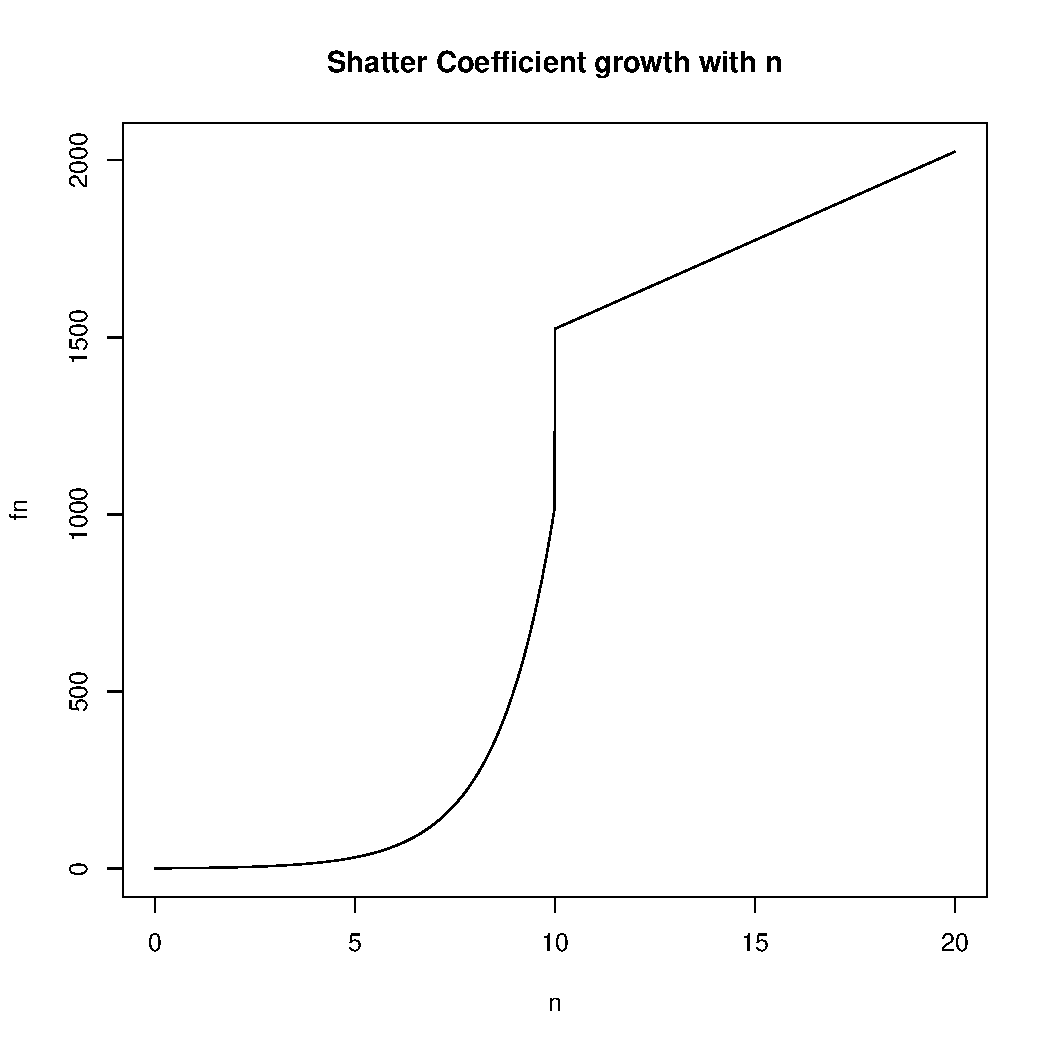
\includegraphics[scale=0.7]{figures/phase_change_shatter_dynamics.pdf}
  \caption[A shatter coefficient plot]{The shatter coefficient function for half spaces in $\mathbb{R}^d$, as a function of $n$. In this plot $d=10$.}\label{fig:phase_change_shatter_dynamics}
\end{figure}

Devroye, Gy\"{o}rfi, and Lugosi \cite{devroye1996probabilistic} provided the following result: 

\noindent \textbf{Theorem 1}\\
For $0<k^2 /(k-1)< n\varepsilon^2$,
\begin{equation}\label{eqn:vcb}
\Pr\left(\underset{A\in \mathcal{A}}{sup} \vert v_n -v\vert > \varepsilon\right) \leq 4ks(\mathcal{A},n)\exp\vspace{-.1in}\left[\frac{-n\varepsilon^2}{2k^2}\right].
\end{equation}

The notation $v_n \overset{def}{=}(1/n)\sum_{i=1}^n\mathds{1}(y_i =\hat{\mathcal{T}}(X_i))$ \newnot{symbol:empirical_error}denotes the empirical error of the estimated classifier and the notation $v\overset{def}{=}\Pr(\mathcal{T}(X)=y)$\newnot{symbol:true_error} denotes the Bayes error of the data. This result tells us that if the family of classifiers has a finite VC dimension, or equivalently a finite shatter coefficient, then the classifier is consistent. Here $k$ and $\varepsilon$ are specified constants, usually we take $k=2$ and $\varepsilon=0.01$. Now we know that a halfspace split in $\mathbb{R}^d$ has $V_\mathcal{A}=d$. Define the entropy function as,\newnot{symbol:entropy}$\mathcal{H}(x) = -xlog(x) -(1-x)log(1-x))$ for $0 \leq x \leq 1$ with $\mathcal{H}(1)=\mathcal{H}(0)=0$. A useful inequality is 

\begin{equation} 
s(\mathcal{A},n)\leq \exp[n\mathcal{H}(V_\mathcal{A}/n)],
\end{equation}
 for $V_\mathcal{A} < 2n$. We see that, for $d<2n$, this inequality holds and, thus, the right hand side of inequality \ref{eqn:vcb} will go to $0$, as $n\to\infty$. For our stump, the tree will capture the Bayes error as $n\to\infty$, if the model is correct. We also see that, for $n<d$, the shatter coefficient for half spaces is $2^n$. If $d\to\infty$ and $n\to\infty$, but $n<d$, we have no consistency guarantee, according to this bound.  In the second case, let us consider a decision tree of arbitrary depth. Theorem 13.5 of Devroye, Gy\"{o}rfi, and Lugosi tells us that for $\mathcal{A} =\{ \mathcal{A}_1 \cap \mathcal{A}_2\}$, 

 \begin{equation}
  s(\mathcal{A},n) \leq s(\mathcal{A}_1,n)s(\mathcal{A}_2,n).
\end{equation}

For decision trees with two splits on halfspaces, the shatter coefficient is bounded above by $2^{2n}=4^n$, for sample sizes less than $d$. For sample sizes larger than $d$ we will have consistency as $n\to\infty$, provided that the decision tree does not grow arbitrarily large. As a simple requirement we ensure that the trees do not grow arbitrarily large, by ensuring that trees are shallower than $K$, for some constant $K$. Note that this constraint was also required by Denison, Mallick and Smith's reversible jump algorithm \cite{denison1998bayesian}. Our simulation studies indicate that there is little to no sensitivity in the specification of $K$. Figures \ref{fig:depth2} -\ref{fig:depth10} show the results of simulating from the posterior distribution over trees and varying the maximum depth, $K$. We evaluate for values of $K=2,3,4,5,6,7,10$. For small values of $K$ such as 2 or 3, the setting of maximum depth appears to limit the sampler from exploring possible trees.  However, once $K$ is set larger than 6, there appears to be little impact restricting the sampler from exploring certain trees. Of course, for any given data set the value of $K$ that is acceptable will likely change, so our conclusion is that $K$ should be large enough. Our assumption is $K=20$ or $K=30$ should be enough for most problems. Simply stated, $K$ should be large. Too small values of $K$ can cause problems. A value of $K=10$ appears sufficient for our purposes and causes no problems. 

  \begin{figure}[h]
  \minipage{0.35\textwidth}%
  \centering
  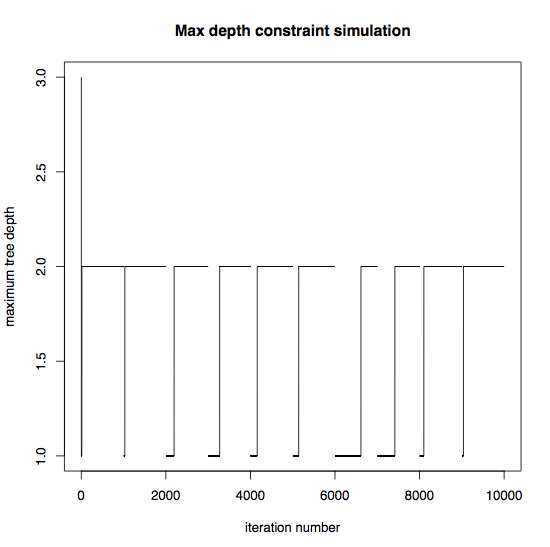
\includegraphics[scale=0.4]{mdepth2.png}
  \caption[Maximum depth of samplers trees with maximum depth set at 2.]{Maximum depth of samplers trees with maximum depth set at 2.}\label{fig:depth2}
\endminipage\hfill
\minipage{0.35\textwidth}%
  \centering
 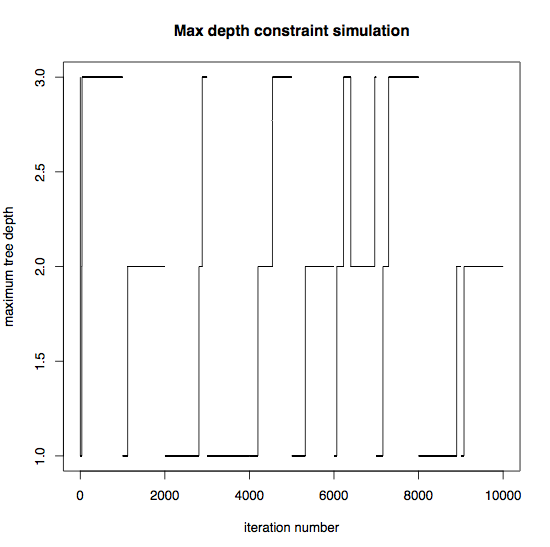
\includegraphics[scale=0.4]{mdepth3.png}
  \caption[Maximum depth of samplers trees with maximum depth set at 3.]{Maximum depth of samplers trees with maximum depth set at 3.}\label{fig:depth3}
\endminipage
\end{figure}

  \begin{figure}[h]
  \minipage{0.35\textwidth}%
  \centering
  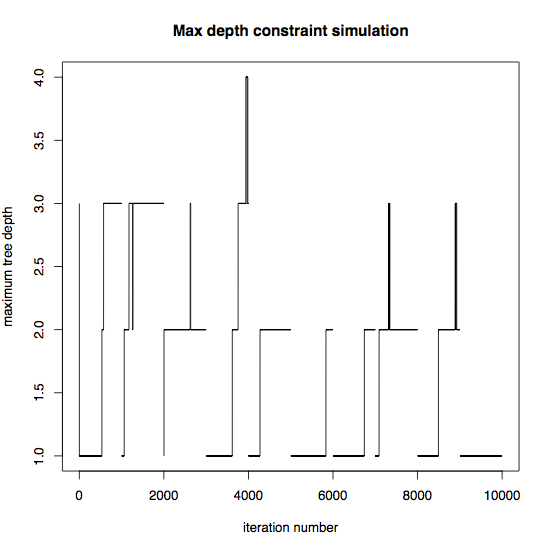
\includegraphics[scale=0.4]{mdepth4.png}
  \caption[Maximum depth of samplers trees with maximum depth set at 4.]{Maximum depth of samplers trees with maximum depth set at 4.}\label{fig:depth4}
\endminipage\hfill
\minipage{0.35\textwidth}%
  \centering
 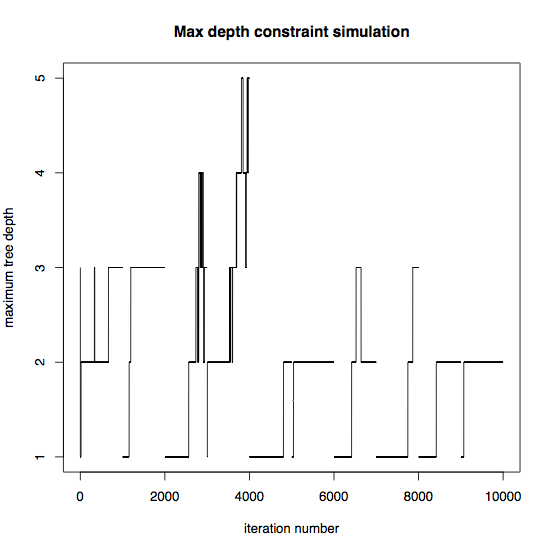
\includegraphics[scale=0.4]{mdepth5.png}
  \caption[Maximum depth of samplers trees with maximum depth set at 5.]{Maximum depth of samplers trees with maximum depth set at 5.}\label{fig:depth4}
\endminipage
\end{figure}

  \begin{figure}[h]
  \minipage{0.35\textwidth}%
  \centering
  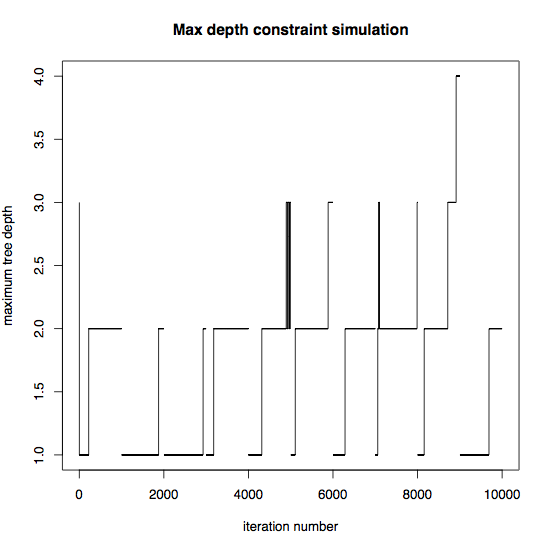
\includegraphics[scale=0.4]{mdepth6.png}
  \caption[Maximum depth of samplers trees with maximum depth set at 6.]{Maximum depth of samplers trees with maximum depth set at 6.}\label{fig:depth6}
\endminipage\hfill
\minipage{0.35\textwidth}%
  \centering
 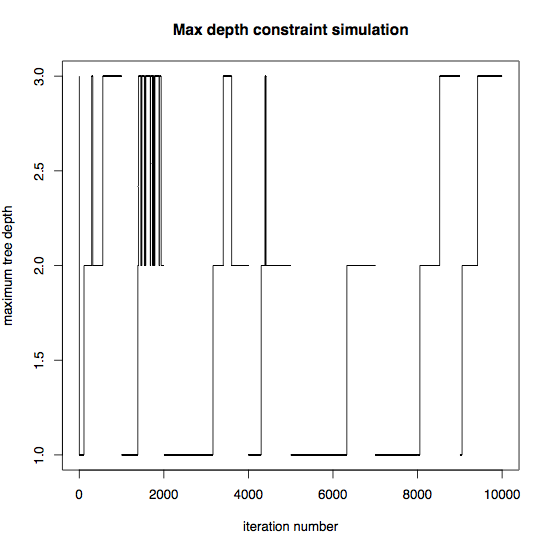
\includegraphics[scale=0.4]{mdepth7.png}
  \caption[Maximum depth of samplers trees with maximum depth set at 7.]{Maximum depth of samplers trees with maximum depth set at 7.}\label{fig:depth7}
\endminipage
\end{figure}

  \begin{figure}[h]
  \centering
  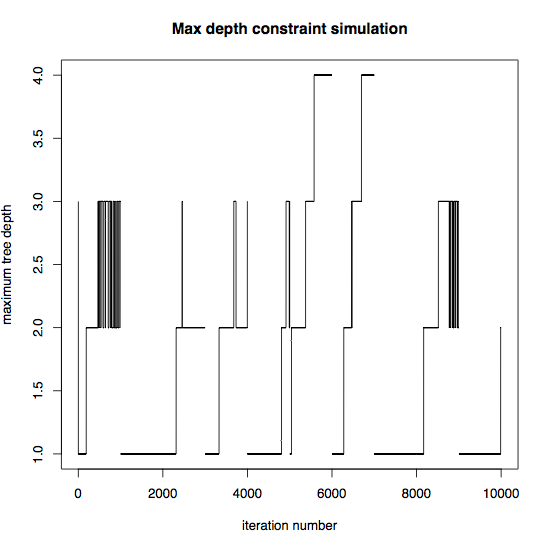
\includegraphics[scale=0.4]{mdepth10.png}
  \caption[Maximum depth of sampled trees with maximum depth set at 10.]{Maximum depth of sampled trees with maximum depth set at 10.}\label{fig:depth10}
\end{figure}


Up to this point, the material in this section is nothing new, but contained fully in the work of Devroye, Gy\"{o}rfi, and Lugosi \cite{devroye1996probabilistic}. Now let us define the sparse shatter coefficient as the shatter coefficient using only dimensions where $S_j =1$, denoted $s(\mathcal{A},n\vert S_{j=1}^d))$ and $S_j \in \{0,1\}$. We now use this sparse definition to carry over results into cases where sparsity holds in classification problems. \\
 
 \textbf{Theorem 2}\\
For $0<k^2 /(k-1)< n\varepsilon^2$ and $\mathbb{E}(S_j)=p_j$, the bound 

\begin{equation}\label{eqn:sparse_vcb}
\small{\Pr\hspace{-.04in}\left(\underset{A\in \mathcal{A}}{sup} \vert v_n -v\vert > \varepsilon\right)\hspace{-.05in} \leq 4ks(\mathcal{A},n\vert S_{j=1}^d))\exp\hspace{-.05in}\left[\frac{-n\varepsilon^2}{2k^2}\right]}
\end{equation} 
holds, if and only if $\sum_{j=1}^dp_j < \infty$, where $d$ can be finite or infinite.
 In the case $d<\infty$ everything looks nearly the same and the proof follows verbatim from the derivation in Devroye, Gy\"{o}rfi, and Lugosi. The case $d=\infty$ is delicate and requires Kolmogorov's three series theorem \cite{loeve1977probability}.    

The second error bound (Equation \ref{eqn:sparse_vcb}) differs from the first (Equation \ref{eqn:vcb}) in that now we are only using some subset of the covariates to classify the observations. Explicitly, the number of effective dimensions, denoted as $d^*$, can be bounded almost surely, but the total number of dimensions $d\to\infty$. Each $S_j \in \{0,1\}$, so if $\Pr(S_j=1)=1$, then we are back into the case of the first theorem, which is non sparse shattering. In our case, we relax the assumption that all $\Pr(S_j=1)=1$ and instead allow $\Pr(S_j=1)=p_j$, for $0\leq p_j\leq 1$. This can be thought of as a convex relaxation of a non-convex, computationally difficult optimization problem. The sum $\sum_j^dS_j$ is now a random sum, since each $S_j$ is a random variable. Also, this random sum is the sparse VC dimension for splits of the form $(\infty, a_i]$, the splits we use to construct our classifiers. Passing to the limit as $d\to \infty$, we want the random infinite series to converge, otherwise we will not have a consistent classifier. The Kolmogorov three series theorem tells us that convergence almost surely of the random series $\sum_{j=1}^\infty S_j$ occurs if and only if the series $\sum_{j=1}^\infty p_j$ converges, thus necessary and sufficient conditions are $\sum_{j=1}^\infty p_j < \infty$. 

We have necessary and sufficient conditions for convergence and therefore for consistency of our sparse classifier in infinite dimensional data. We need only ensure that $\sum_{j=1}^\infty p_j < \infty$. Provided $\sum_{j=1}^\infty p_j <\infty$ the stump tree will be consistent with infinite dimensional data as $n\to\infty$ Furthermore, the tree with arbitrary but finite depth will also be consistent, provided that the tree does not grow too deep, less than $2^K$ for some large but finite $K$. Intuitively this result should make sense. For infinite dimensional data, we must have most dimensions be irrelevant for the classification task, in order for the resulting classifiers to be consistent. In other words, most $p_j \to 0$ and some $p_{j^\prime}\to c >0$ ($0<c<1$) as $d\to\infty$. Our approach, without the $\widetilde{\alpha}$, ensures precisely this condition. Furthermore, this is not a weakness of our approach, because this theoretical result holds for $d\to\infty$. In our real data cases $d$ is finite and usually fixed. The $\widetilde{\alpha}$ is a practical aspect of our approach and is used to improve exploration and exploitation in fixed, finite dimensional data. 

\subsection{A Simulated Example}\label{sec:ase}

This section details a simulated example where we know which covariates are important and which are not important. Of course, this will never be the case in practice, yet, for verification, we find this setting useful. 

For our example, we note that a greedily built decision tree with a linear classifier can universally fail, if we are willing to make $d$ large enough. To accomplish this for each covariate after $d^*$, we will simulate from a mixture of two normals, where each mixing probability is $1/2$, and the means of the two normals are taken from a continuous uniform distribution on a large enough region $(l,u)$. If we can generate data where each covariate has observations in two groups that are separated enough and some of the responses are also separated, then we will incorrectly select a split rule based on this covariate, when in reality this covariate is independent of the response by construction. This will occur more frequently for larger $d$. Fortunately, our method will still select the correct covariates and as a result, select the correct tree.   

 Let us define the data generating process (DGP)\newabbrev{abbrev:DGP} as that given in Figure \ref{fig:awesome_image2}.  

\begin{figure}[h]
\centering
\label{fig:3fig_tree}
  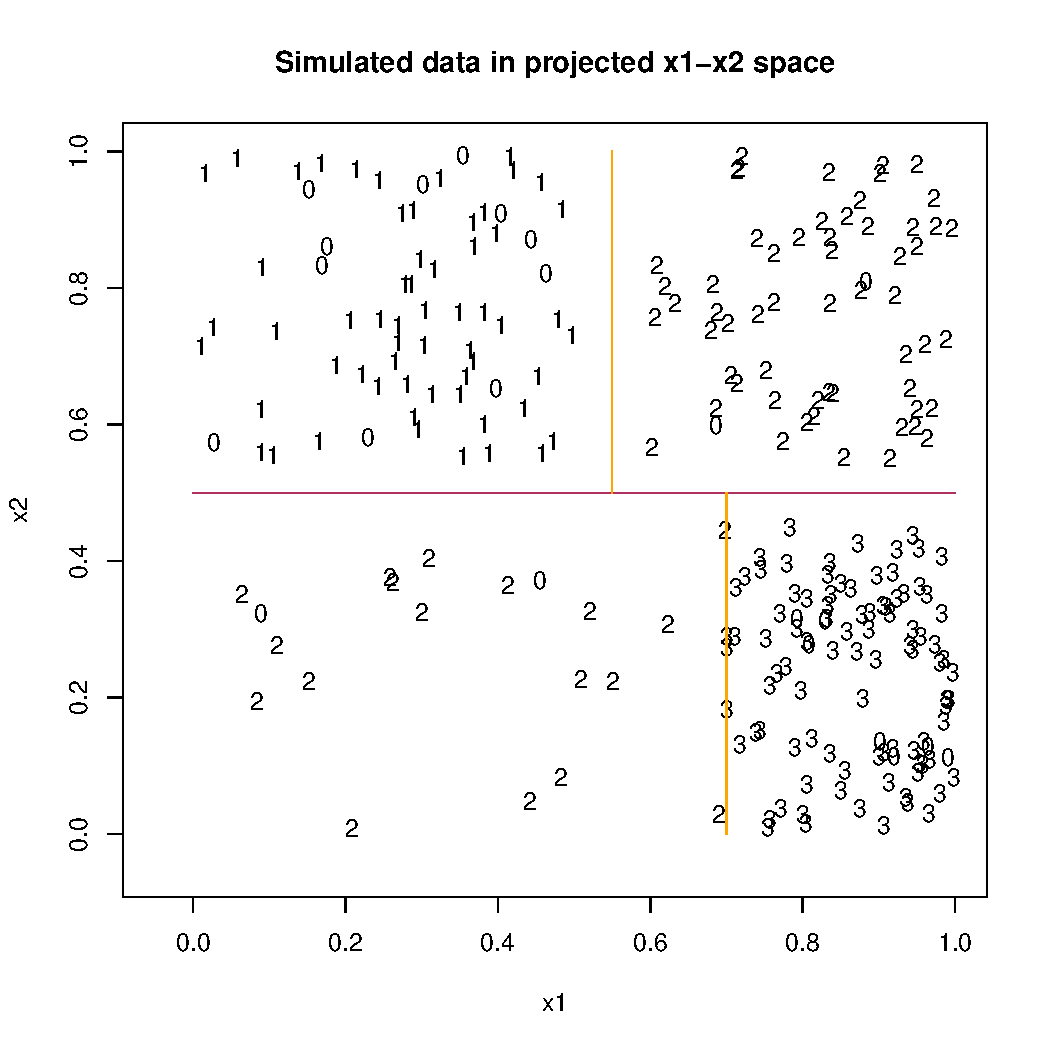
\includegraphics[scale=0.4]{figures/proj_plot.pdf}
  \caption{A plot of the true DGP}\label{fig:awesome_image2}
\end{figure}

The probability of being the majority class in any of the four regions of the Figure \ref{fig:awesome_image2} is 90\%. Therefore no perfect classifier exists, yet very good classifiers are possible. We next generate additional covariates independently according to the mixture strategy described in the previous paragraph, with the continuous uniform supported on the interval $(0,20)$. We look at the cases of $d=100 \text{ and } 400$. The trees generated by the three tree methods are shown in Figures \ref{fig:awesome_image1}-\ref{fig:awesome_image3}. The best tree found by our method is the generative tree of the data, and therefore this classifier achieves the Bayes error rate for this example. We simulate several Markov chains are simulated to guard against trapping in local optima. This is not a new strategy for MCMC with many local optima and was proposed by CGM \cite{chipman1998bayesian} for decision tree MCMC samplers to aid exploration of the decision tree space and to prevent getting stuck in one of the many local optima.  We tried a few chain lengths (500, 1000, and 2000) of each chain and fitted 10 chains on each data set. The results were the same, regardless of the chain length.

\begin{figure}[h]
\centering
\label{fig:3fig_tree}
  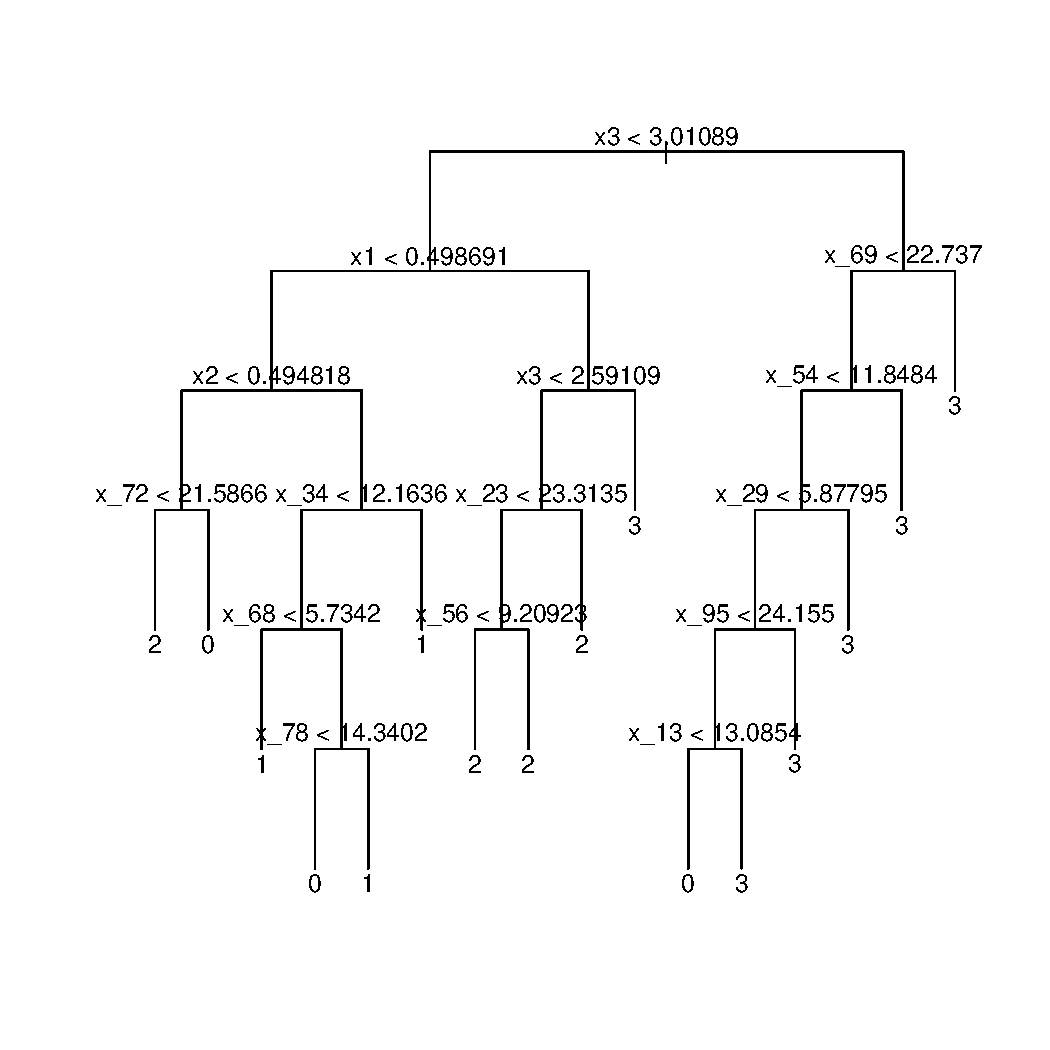
\includegraphics[scale=0.4]{threetree1.pdf}
  \caption{The tree found by a greedy optimization.}\label{fig:awesome_image1}
  \end{figure}
  \begin{figure}[h]
  \minipage{0.35\textwidth}%
  \centering
  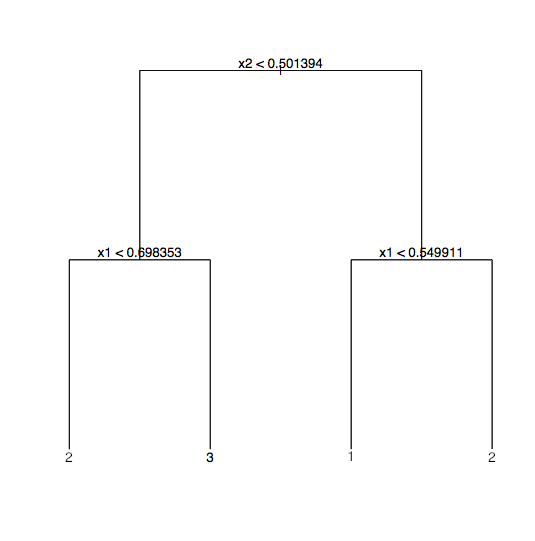
\includegraphics[scale=0.4]{figures/simul_example_map_tree_USE.png}
  \caption{The best tree using the weighted method.}\label{fig:awesome_image4}
\endminipage\hfill
\minipage{0.35\textwidth}%
  \centering
 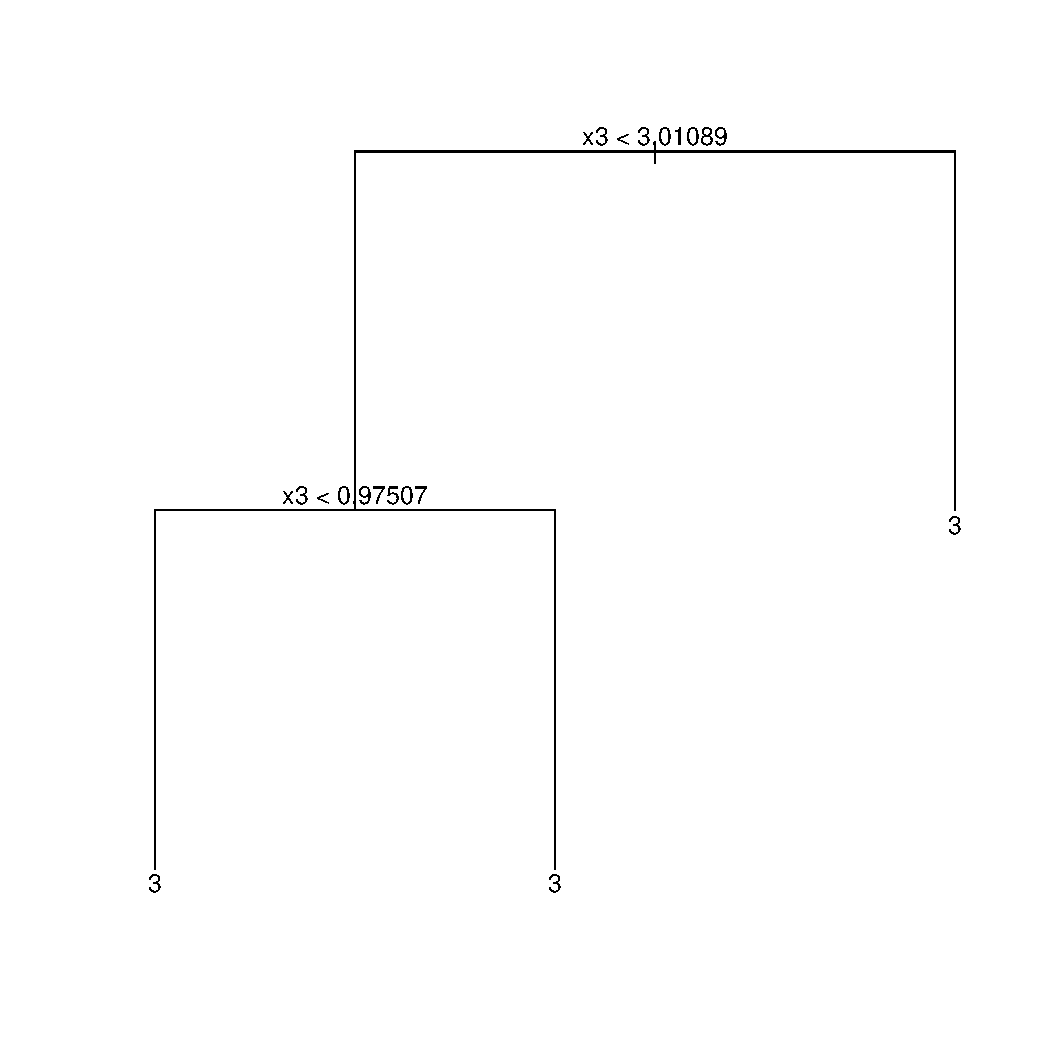
\includegraphics[scale=0.4]{figures/cgm_tree_simul.pdf}
  \caption{The best tree found by the CGM method.}\label{fig:awesome_image3}
\endminipage
\end{figure}
\begin{figure}[h]
\centering
\label{fig:3fig_tree}
\minipage{0.35\textwidth}
\centering
  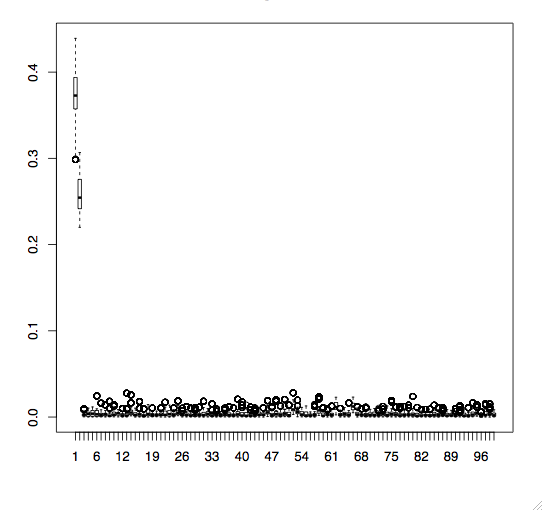
\includegraphics[scale=0.4]{figures/weight_simulated_example_USE1.png}
  \caption[Covariate inclusion probabilities for the 100 covariate example.]{Covariate weights on the 100 dimensional example. Note the first two covariates are selected with high probability and the rest with miniscule probability.}\label{fig:awesome_image5}
\endminipage\hfill
\minipage{0.35\textwidth}
\centering
  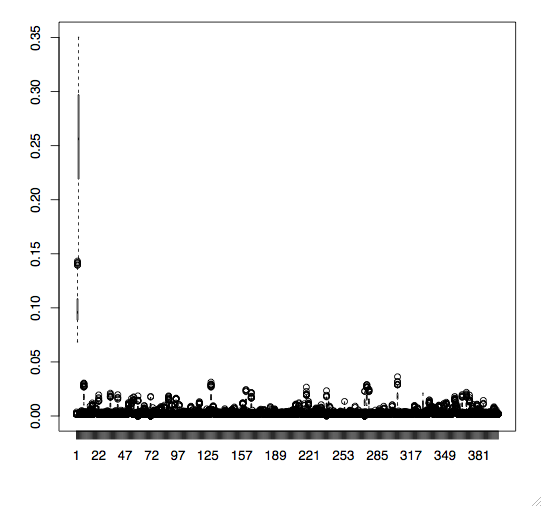
\includegraphics[scale=0.4]{figures/my_method1.png}
  \caption[Covariate inclusion probabilities for the 400 covariate example.]{Covariate weights on the 400 dimension simulated example. Note the first two covariates are selected with high probability and the rest with negligible probability.}\label{fig:awesome_image6}
\endminipage\hfill
\end{figure}
\begin{table}[h]\footnotesize
\centering
  \begin{tabular}{| c | c | c }
  \hline 
Method & Misclass Prob.\\
      \hline 
Greedy &   11.6\%    \\
 CGM &     62.4\% \\
   Weighted & 10.8\%   \\
      \hline
  \end{tabular}
    \caption[Misclassification probabilities for $d=100$.]{Misclassification probabilities of the three tree fitting methods for $d=100$.}
  \label{tab:sim_misclass1}
\centering
\end{table}

\begin{table}[h]\footnotesize
\centering
  \begin{tabular}{| c | c | c }
  \hline 
Method & Misclass Prob.\\
      \hline 
Greedy &  24.8\%     \\
 CGM &    57.2\% \\
   Weighted &  10.0\%  \\
      \hline
  \end{tabular}
    \caption[Misclassification Probabilities of the three tree fitting methods for $d=400$]{Misclassification Probabilities of the three tree fitting methods for $d=400$.}
  \label{tab:sim_misclass2}
\centering
\end{table}


To compare the three methods, we calculate misclassification probabilities for each of the three methods. We took a random sample of 250 observations as hold out, or test data, to calculate misclassification probabilities. The misclassification probabilities are calculated by dropping all data points from the test data set through the resulting trees. We fit the trees using only the 250 observations from the training data. The tables of misclassification probabilities are displayed in Tables \ref{tab:sim_misclass1} and \ref{tab:sim_misclass2}.

We see that the pruning rule fails to collect the correct covariates as important in the greedily grown tree. The problem is that the deterministic procedure is overwhelmed by candidate splits and thus overfits. In fact, the misclassification probability \emph{within} the training data is 4.8\%, better than the Bayes rate! However, this method performed poorly on hold out data compared to the weighted method, as shown in Tables \ref{tab:sim_misclass1} and \ref{tab:sim_misclass2}. The greedy method eventually finds some suboptimal splits. Of course, in this example we know the truth, and these extra splits are far from the truth. In addition, we see that the CGM approach fails on these trees. Much like the greedy method, the CGM approach is also overwhelmed with possible splits. Each new covariate adds exponentially more possible trees. This plethora of trees often allows one to find many locally optimal trees, but at the cost of exponentially increased search time. A benefit of our method is the improved search by effectively ignoring certain covariates and preventing some trapping of the chain in local optima. By allowing non-uniform probabilities of selecting covariates, the algorithm spends more time searching through covariates that have good splits, while not spending time in other covariates that have mostly useless splits. This behavior leads to a more efficient search of the tree space and, consequently, better predictive trees than those found by the CGM search approach. The trees built using our weighted approach are better or competitive in prediction but simpler for inference compared with those found by a greedy search as indicated by the results in Table \ref{tab:sim_misclass2}. 

\subsubsection{Choosing Covariates}
A natural question to ask is: How should one choose covariates? This question is important because there are often covariates which have estimated probabilities that might be considered large enough to be important but also could be small enough to be considered   not important. We approach this question from the context of the learning achieved during the sampling. We call the prior moment estimator defined here by Equation \ref{eqn:mom_est_dirichlet} as

\begin{equation}\label{eqn:mom_est_dirichlet}
\Pr(\text{covariate $j$ included})= \frac{\alpha_j}{\sum_{j=1}^d \alpha_j}.
\end{equation}

Nonetheless, the prior moment estimator does not take into account the learning performed by the MCMC algorithm. We now discuss a method that accounts for the learning occurring as the MCMC algorithm progresses.

Note that Equation \ref{eqn:mom_est_dirichlet} is simply the maximum likelihood estimator of the \emph{a priori} probabilities of each covariate being selected to split on in the decision tree. To choose which covariates to use (in some subsequent model building), one might select those covariates where the \emph{a posteriori} probabilities are larger than the \emph{a priori} probabilities. This then indicates that information on the covariates was learned during the course of the MCMC algorithm. Formally, select the set of covariates for inclusion according to the rule 

\begin{equation}\label{eqn:cov_inclusion_rule}
 J = \left\{ \text{all } j:\frac{\alpha^\prime_j}{\sum_{j=1}^d\alpha^\prime_j}>  \frac{\alpha_j}{\sum_{j=1}^d\alpha_j } \right\},
\end{equation}
where the $\alpha_j^\prime = \alpha_j +\widetilde{\alpha}s_j$ denote posterior concentration parameters for each covariate.
 
 Other methods for covariate selection are possible but we do not discuss them here. 
We present a small simulation study to determine the efficacy of the proposed method. We simulate data as described in the earlier portion of this section, where we know the specified covariates that should be selected, and those that should not. We ran the simulation 100 times and present the average percentage correctly selected by using the rule in Equation \ref{eqn:cov_inclusion_rule} for our weighted method. We also compared our weighted method results to simple frequency estimates using bootstrap samples and using the CGM method for fitting decision trees. The results are presented in Table \ref{tab:sim_study}. We fit a collection of trees using a bootstrap resample of 100 and using 1000 trees and calculate the number of times the correct covariates are selected. These entries are the subscripted `100' and `1000' entries in Table \ref{tab:sim_study}. 

% \begin{table}[h]\centering
%  \begin{tabular}{| c | c  c  c  c  c |}  \hline 
%
%      \hline 
%$\Pr(\text{covariate 1 selected})$ & - & - & - & - & - \\
%$\Pr(\text{covariate 2 selected})$&  - & - & - & - & - \\
% $\Pr(\text{ covariates 1 and 2 selected})$&  - & - & - & - & - \\
%$\Pr(\text{any other covariates  selected})$&  - & - & - & - & - \\
%   \hline
%  \end{tabular}
%  \caption{The empirical performance of the tree fitting methods on the variable selection problem using 100 simulations.}
%  \label{tab:sim_study}
%\centering
%\end{table}

% latex table generated in R 2.15.0 by xtable 1.7-0 package
% Thu Feb 21 09:12:06 2013

\begin{table}[ht]
\begin{center}
\begin{tabular}{l | rrrrr}
  \hline
  & Weights & Boot$_{100}$ & Boot$_{1000}$ & Greedy & CGM \\ 
  \hline
$\Pr(\text{covariate 1 selected})$ & 0.32140 & 0.12405 & 0.12664 & 0.12178 & 0.13333 \\ 
$\Pr(\text{covariate 2 selected})$ & 0.33806 & 0.10795 & 0.10835 & 0.12376 & 0.06667 \\ 
  $\Pr(\text{covariates 1 and 2 selected})$& 0.15429 & 0.08712 & 0.08365 & 0.08614 & 0.06667 \\ 
  $\Pr(\text{any other covariates  selected})$ & 0.34054 & 0.76799 & 0.76502 & 0.75446 & 0.80000 \\ 
   \hline
\end{tabular}
 \caption[Empirical covariate selection with 100 simulations]{The empirical performance of the tree fitting methods on the variable selection problem using 100 simulations.}
 \label{tab:sim_study}
 \end{center}
\end{table}


From Table \ref{tab:sim_study} it is clear that the weighted method outperforms the four other methods in correctly selecting the important covariates. Also, our weighted method selects the correct covariates jointly better than the other methods. Moreover, our weighted method selects incorrect covariates less often than the other method. It is important to note that theoretically we do not want the entries in the last line to approach zero. If we did this then the MCMC would get immediately stuck in a local maximum of the likelihood space and would not find many good local maxima. Our weighted method is able to more evenly balance the search for new local maxima with the search for the correct splits and tree topology within the basin of attraction of the current local maximum. Weighting the covariates leads to improved searching of the tree space and leads to better trees in terms of inference, which are competitive in terms of prediction.  

\section{A Case Study of the DiVaS Model}\label{sec:real_data}
In this section we compare our method against the greedy approach and the CGM approach using the publicly available internet ads dataset from the UCI data repository \cite{Frank:2010uq}. The internet ads data set contains 1558 covariates, some numeric and some categorical. The data set was first used in a paper by Kushmerick \cite{kushmerick1999learning} and has since been used in several statistical classification studies. The UCI machine learning repository contains a more complete listing of papers using this dataset. 

As noted by Kushmerick \cite{kushmerick1999learning}, there are several reasons for wanting to remove advertisements from webpages. Some reasons are: Images tend to dominate a page�s total download time, users dislike paying for services indirectly through advertisers, preferring direct payment for services rendered, and malicious software can be unintentionally placed on a user's machine through images masked as advertisements. 

We used a random subset of internet advertisements data to fit a greedy tree, a CGM tree, and a tree fit using our weighted method. We first removed all observations that contain missing values. We then took a 50\% random sample of training and test data. Figures \ref{fig:ads_image1}-\ref{fig:ads_image3} plot the fitted trees. The misclassification probabilities are calculated by dropping all data points from the test data set through the trees built using the training data. The resulting trees are fit using only the training data.  
\begin{figure}[h]
\label{fig:3fig_tree}
\minipage{0.35\textwidth}
  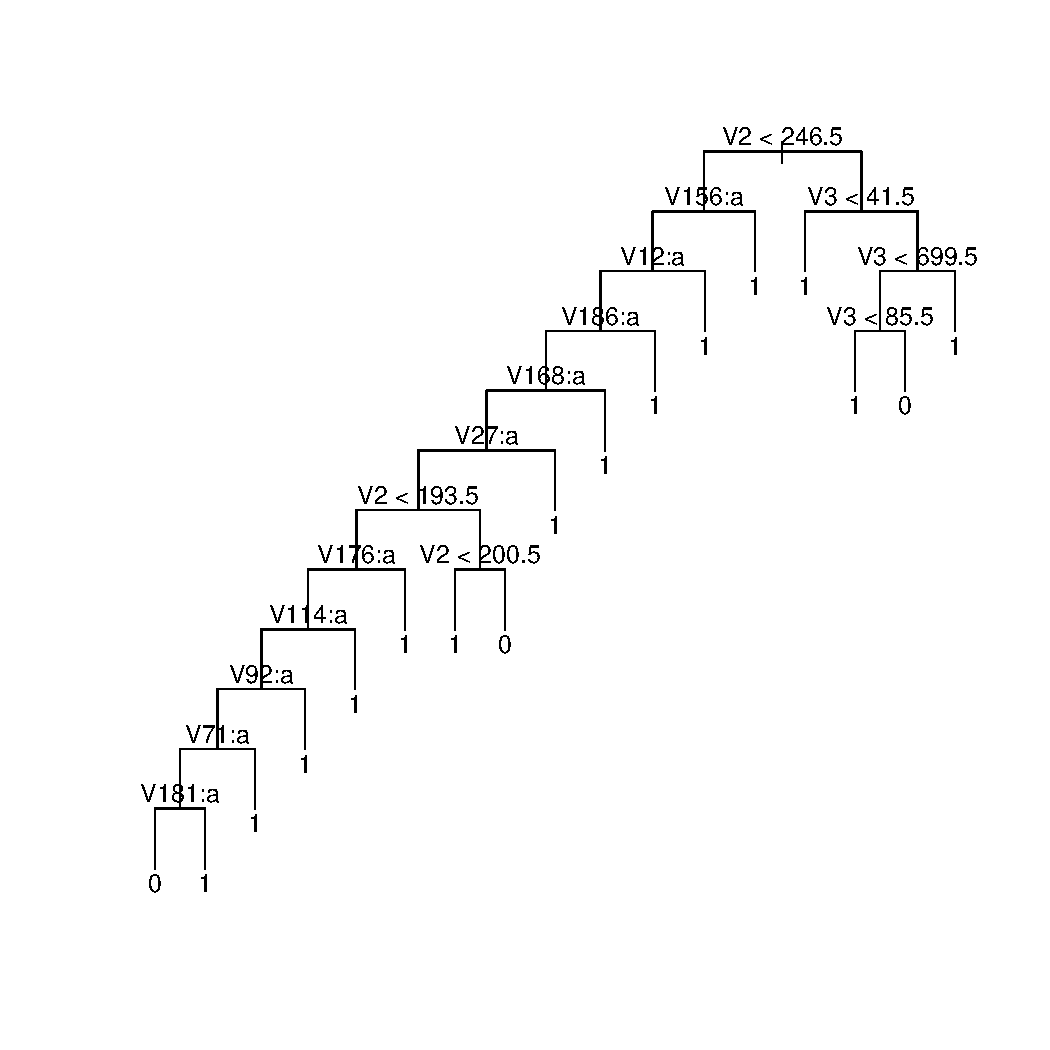
\includegraphics[scale=0.4]{ad_tree.pdf}
  \caption[The greedy algorithm tree for the internet ads dataset]{The greedy tree.}\label{fig:ads_image1}
\endminipage\hfill
\minipage{0.35\textwidth}
  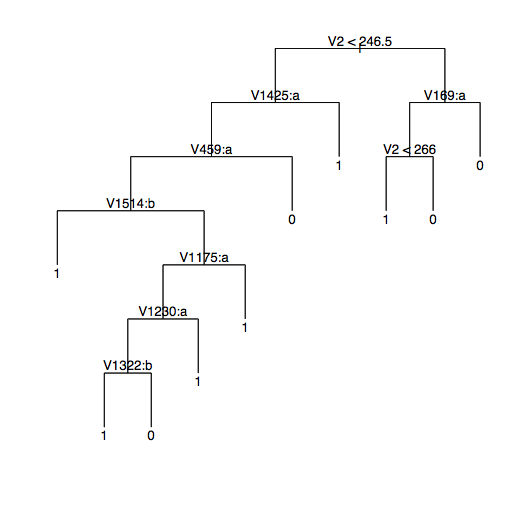
\includegraphics[scale=0.4]{CGM.png}
  \caption[The CGM algorithm tree for the internet ads dataset]{The tree found by the CGM algorithm on the internet ads dataset.}\label{fig:ads_image2}
\endminipage\hfill
\end{figure}
\begin{figure}
\minipage{0.35\textwidth}%
  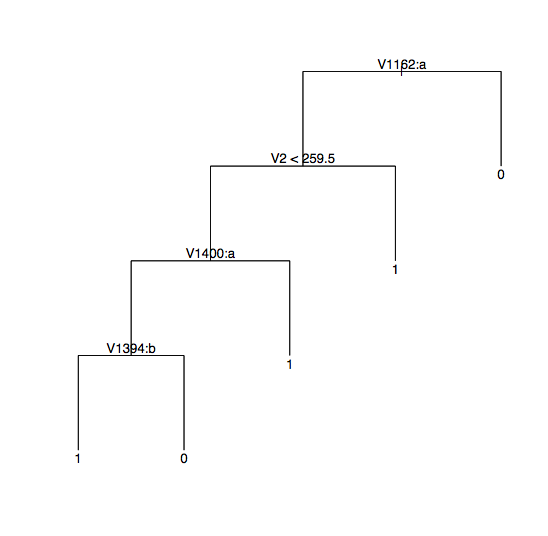
\includegraphics[scale=0.4]{estim2_tree.png}
  \caption[The weighted method tree for the internet ads dataset]{Best tree using the weighted method on the internet ads dataset.}\label{fig:ads_image3}
\endminipage\hfill
\minipage{0.35\textwidth}%
  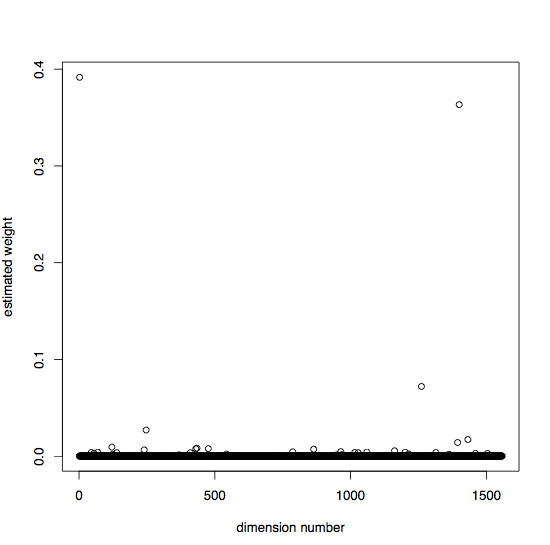
\includegraphics[scale=0.4]{weights_estim2.png}
  \caption[Estimated covariate weights for the internet ads dataset]{Estimated covariate weights using the internet ads dataset.}\label{fig:ads_image4}
\label{fig:uci_cov_weights}
\endminipage
\end{figure}
\begin{table}[h]\footnotesize
\centering
  \begin{tabular}{| c | c | c }
  \hline 
Method & Misclass Prob.\\
      \hline 
Greedy & 5.578\% \\ %0.0557598      \\
 CGM &   7.2\% \\%.0716912   \\
   Weighted & 5.598\% \\%0.0559853   \\
      \hline
  \end{tabular}
    \caption[Misclassification probabilities for internet ads dataset]{Misclassification probabilities of the three tree fitting methods on the internet ads dataset.}
      \label{tab:misclass_uci}
\centering
\end{table}

% latex table generated in R 2.15.0 by xtable 1.7-0 package
% Thu Feb 21 12:06:56 2013

\begin{table}[ht]
\hspace{-.7in}
\begin{tabular}{r|rrrrrrrrrrrrrrrrrrrrrrrrrrrrrrrrrrrr}
  \hline
 Cov Num & 2$^*$ & 1400$^*$ & 1261 & 247 & 1432 & 1394$^*$ & 121 & 434 & 476 & 430 & 864 & 240 \\
 Rank & 607.78$^*$ & 563.94$^*$ & 111.91 & 42.00 & 26.78 & 21.99$^*$ & 14.66 & 12.97 & 12.12 & 11.84 & 11.28 & 10.15 \\
 \hline
Cov Num & 1162$^*$ & 964 & 787 & 1060 & 69 & 1201 & 45 & 1015 & 1314 & 139 & 410 & 1028 \\ 
 Rank   & 8.74$^*$ & 7.33 & 7.05 & 6.77 & 6.48 & 6.48 & 5.92 & 5.92 & 5.92 & 5.64 & 5.64 & 5.64\\
 \hline
 Cov Num& 55 & 1460 & 1504 & 1214 & 543 & 123 & 1362 & 967 & 368 & 949 & 253 & 813 \\ 
  Rank   & 4.79 & 4.51 & 4.51 & 3.66 & 3.38 & 3.10 & 3.10 & 2.54 & 2.26 & 2.26 & 1.41 & 1.13 \\ 
   \hline
\end{tabular}
\caption[The set $J$ of covariates using Equation \ref{eqn:cov_inclusion_rule}]{The set $J$ of possibly included covariates from Equation \ref{eqn:cov_inclusion_rule}. Covariates are listed in decreasing order of the value used to include them in $J$. Stars indicate covariates used in Figure \ref{fig:ads_image3}. The rank is a numeric value that follows from Equation \ref{eqn:cov_inclusion_rule}.  }
\label{tab:ads_data_ranks}

\end{table}

Table \ref{tab:misclass_uci} shows that the best tree both in terms of simplicity, and in terms of misclassification probabilities, is the tree fir using our weighted method. The CGM approach is not as good at predicting as the trees found by either the greedy or our weighted approach. Amongst the weighted and greedy approaches, the tree found by the greedy algorithm is far more complex than the tree found by our weighted method. The weighted method is essentially as good in terms of prediction error as the greedy method and is simpler to understand and interpret. Moreover, the greedy method and the CGM method do not provide output explicitly indicating which covariates are useful in the model.

Figure \ref{fig:uci_cov_weights} presents the estimated  probability of selection from our model. In this case there are three covariates that are clearly important in the model. Table \ref{tab:ads_data_ranks} ranks the covariates selected according to the rule from Equation \ref{eqn:cov_inclusion_rule} in decreasing order. The covariates used in the tree in Figure \ref{fig:ads_image3} correspond to a subset of these covariates and are starred in the table. The starred covariates are: the width of the image, the url tag ``tkaine+bars'', the url tag ``www.irish-times.com'', and the url tag ``click''. The tag ``click'' is not particularly surprising because many ads are in the form of images that pop up a secondary webpage if you click on the image. The ``Irish Times'' is a newspaper and a perusal of their current webpage indicates that they have many images that accompany news articles and we can reasonable assume the website was similar when the dataset was created. The width field is also not surprising, wide windows facilitate better views of images. It is not very clear what the field ``tkaine+bars'' means. Perhaps some of the images come from a collection of webpages during Tim Kaine's race for mayor of Richmond, Virginia, in 1998. Admittedly, more information on this field would be desirable. 
 
\subsection{Discussion of Results}\label{sec:conc}
In this chapter we studied the application of MCMC data partitioning models to large dimensional data. We showed that, in large dimensional data sets, the methods used on low dimensional examples will not work effectively. We provided a simple modification that greatly improves the accuracy and utility of the partitioning scheme in large dimensional datasets. 

 When running MCMC algorithms on large dimensional data, we spend more time searching the covariates that are important (high probability) and ignoring the covariates that are not useful (the low probability ones). Moreover, the values of the probabilities for each covariate are on a probability scale providing intuitive interpretation of the values sampled from the posterior distribution of weights.
Sparsifying our tree search procedure provides us with several benefits. Firstly, we are able to separate the covariates into groups of high and low probability. Secondly, this gives us simplified interpretation of the tree models by searching for simple trees and eases inference for the analyst. Thirdly, we explore the state space more efficiently than the nonsparse greedy approach or the CGM search approach. 

Finally, we note that our approach to sparsity is different from the approach in Chipman, George and McCulloch \cite{chipman2000hierarchical}. In their work the goal was to model using short trees, so sparsity was achieved as a byproduct of constraining the complexity of the decision tree. Furthermore, a simple tree was their primary goal and no measure of usefulness on each covariate was desired. The inferential difficulties of the pruning rule noted in the introduction still apply to the Chipman et al. \cite{chipman2000hierarchical} method, whereas our dimension weighting does not have this difficulty. 

%\subsubsection*{Acknowledgements}
%We would like to thank Dr. Robert Gramacy for clarification of several aspects of his papers and for the referees for their comments which improved on an early draft of this paper. 
%\subsubsection*{References}

